\documentclass{article}
\usepackage[utf8]{inputenc}
\usepackage{subfig}
\usepackage{amsmath}
\usepackage[export]{adjustbox}
\usepackage{graphicx}
\usepackage[legalpaper, landscape, margin=0.5cm]{geometry}

\thispagestyle{empty}
% \renewcommand{\thesubfigure}{\roman{subfigure}}
\begin{document}

\begin{figure}[h]
        \centering
        \subfloat[]{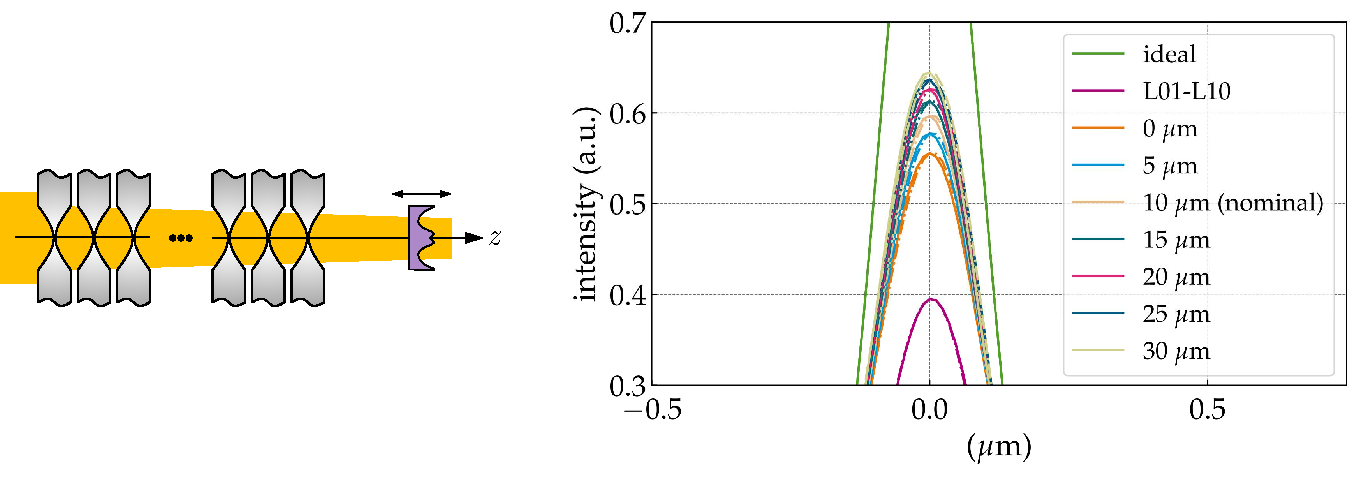
\includegraphics[height=4.5cm]{figures/ch06/longitudinal.pdf}}
        \subfloat[]{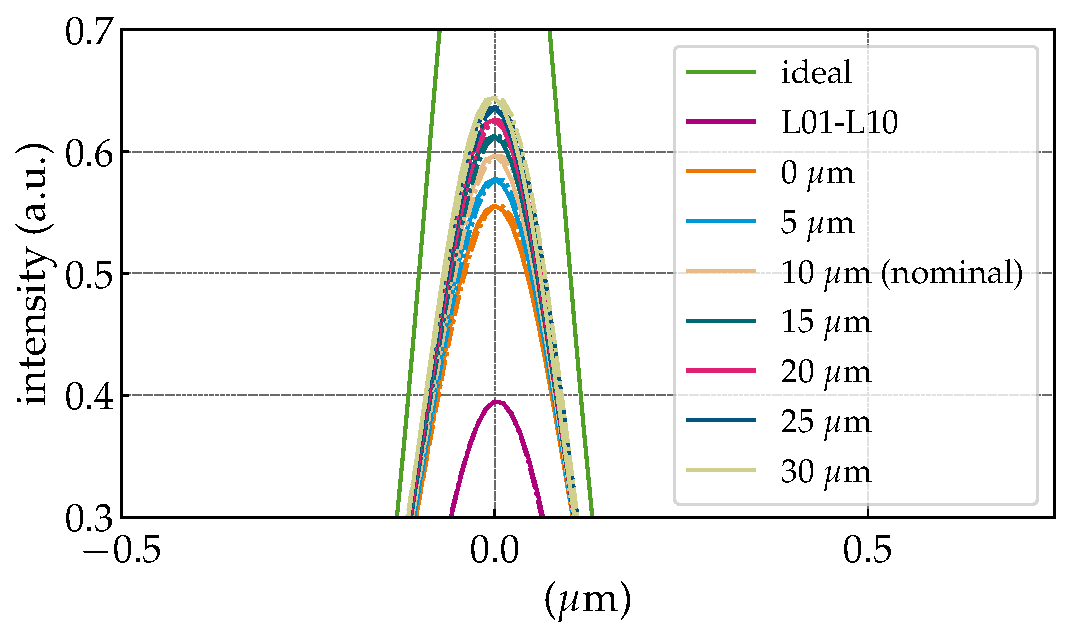
\includegraphics[height=4cm]{figures/ch06/longitudinal_scan.pdf}}\\
        \caption*{longitudinal scan}
        \subfloat[]{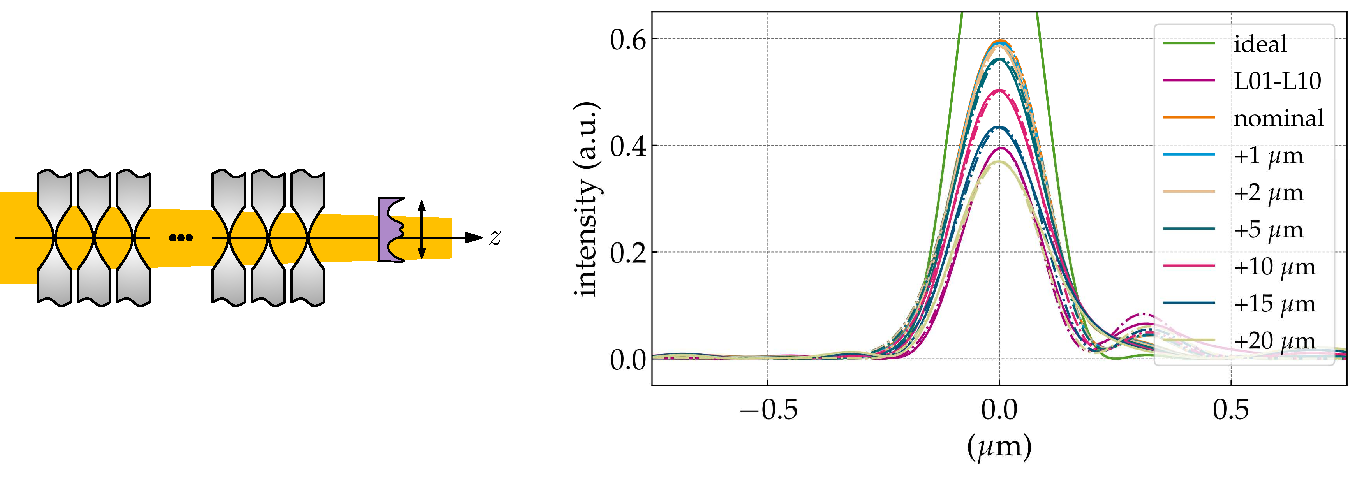
\includegraphics[height=4.5cm]{figures/ch06/transverse.pdf}}
        \subfloat[]{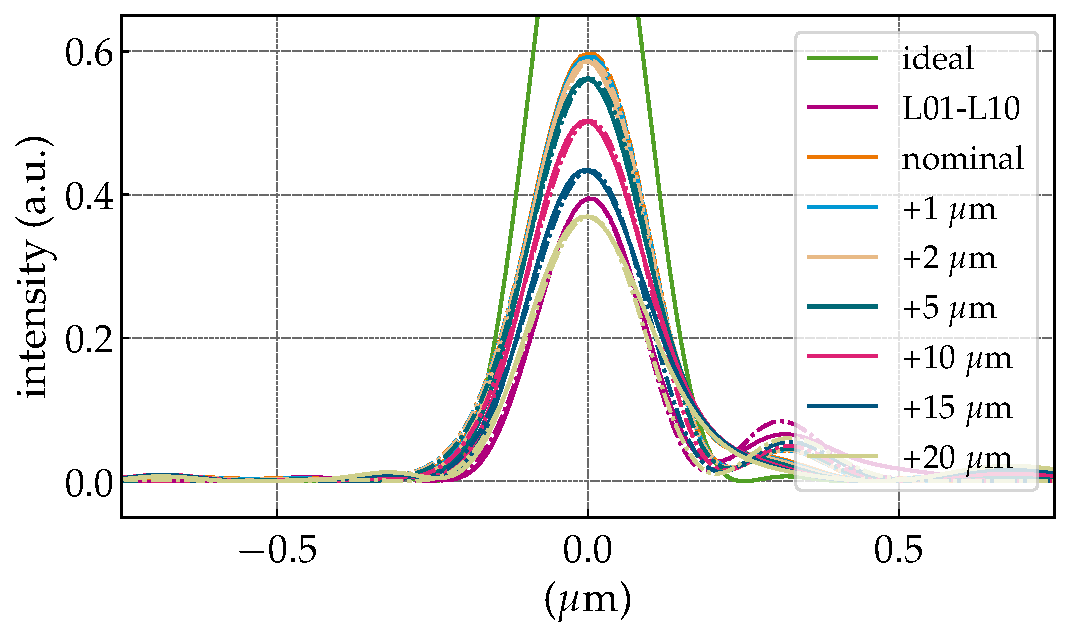
\includegraphics[height=4cm]{figures/ch06/lateral_scan.pdf}}\\%\hspace{0.1cm}
        \caption*{transverse scan}
        \subfloat[]{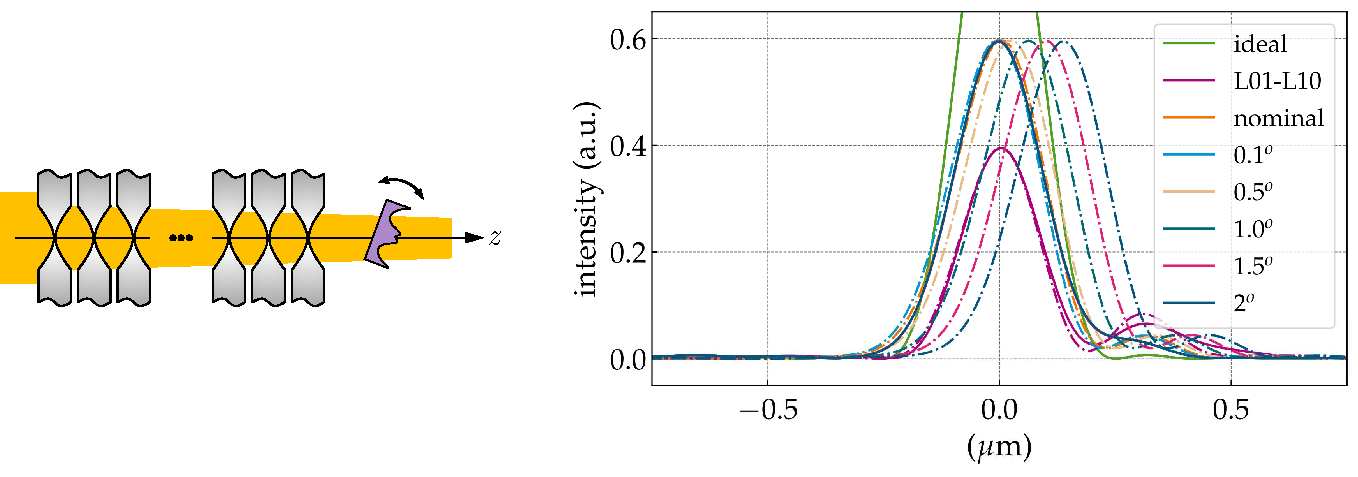
\includegraphics[height=4.5cm]{figures/ch06/angular.pdf}}
        \subfloat[]{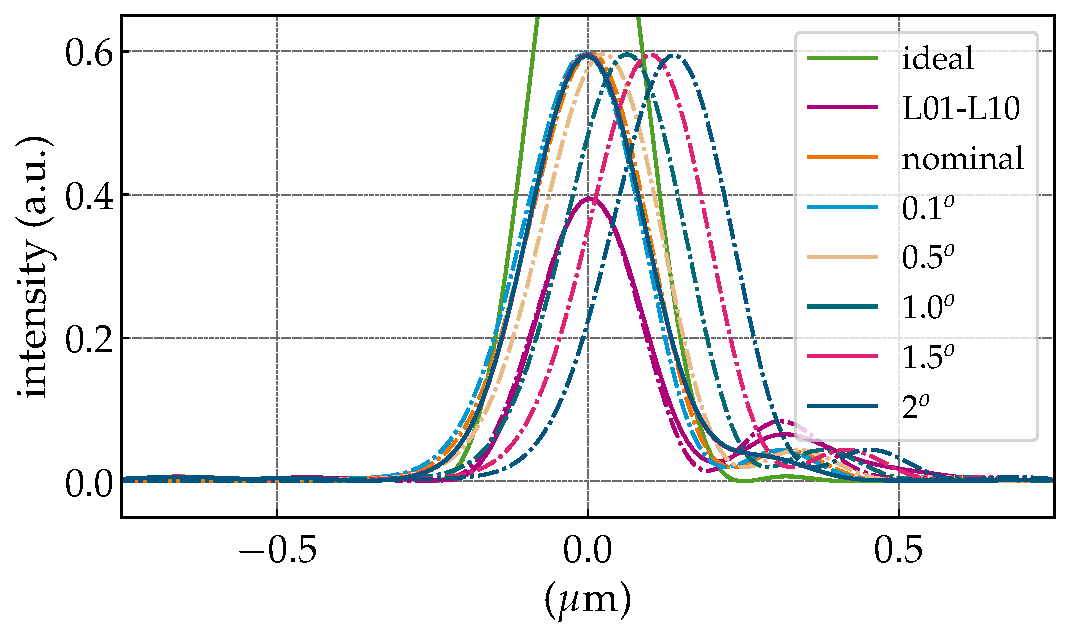
\includegraphics[height=4cm]{figures/ch06/angular_scan.pdf}}
        \caption*{angular scan}


\end{figure}
\end{document}